% Options for packages loaded elsewhere
\PassOptionsToPackage{unicode}{hyperref}
\PassOptionsToPackage{hyphens}{url}
%
\documentclass[
  twocolumn]{article}
\usepackage{lmodern}
\usepackage{amssymb,amsmath}
\usepackage{ifxetex,ifluatex}
\ifnum 0\ifxetex 1\fi\ifluatex 1\fi=0 % if pdftex
  \usepackage[T1]{fontenc}
  \usepackage[utf8]{inputenc}
  \usepackage{textcomp} % provide euro and other symbols
\else % if luatex or xetex
  \usepackage{unicode-math}
  \defaultfontfeatures{Scale=MatchLowercase}
  \defaultfontfeatures[\rmfamily]{Ligatures=TeX,Scale=1}
\fi
% Use upquote if available, for straight quotes in verbatim environments
\IfFileExists{upquote.sty}{\usepackage{upquote}}{}
\IfFileExists{microtype.sty}{% use microtype if available
  \usepackage[]{microtype}
  \UseMicrotypeSet[protrusion]{basicmath} % disable protrusion for tt fonts
}{}
\makeatletter
\@ifundefined{KOMAClassName}{% if non-KOMA class
  \IfFileExists{parskip.sty}{%
    \usepackage{parskip}
  }{% else
    \setlength{\parindent}{0pt}
    \setlength{\parskip}{6pt plus 2pt minus 1pt}}
}{% if KOMA class
  \KOMAoptions{parskip=half}}
\makeatother
\usepackage{xcolor}
\IfFileExists{xurl.sty}{\usepackage{xurl}}{} % add URL line breaks if available
\IfFileExists{bookmark.sty}{\usepackage{bookmark}}{\usepackage{hyperref}}
\hypersetup{
  hidelinks,
  pdfcreator={LaTeX via pandoc}}
\urlstyle{same} % disable monospaced font for URLs
\usepackage[margin=1in]{geometry}
\usepackage{longtable,booktabs}
% Correct order of tables after \paragraph or \subparagraph
\usepackage{etoolbox}
\makeatletter
\patchcmd\longtable{\par}{\if@noskipsec\mbox{}\fi\par}{}{}
\makeatother
% Allow footnotes in longtable head/foot
\IfFileExists{footnotehyper.sty}{\usepackage{footnotehyper}}{\usepackage{footnote}}
\makesavenoteenv{longtable}
\usepackage{graphicx,grffile}
\makeatletter
\def\maxwidth{\ifdim\Gin@nat@width>\linewidth\linewidth\else\Gin@nat@width\fi}
\def\maxheight{\ifdim\Gin@nat@height>\textheight\textheight\else\Gin@nat@height\fi}
\makeatother
% Scale images if necessary, so that they will not overflow the page
% margins by default, and it is still possible to overwrite the defaults
% using explicit options in \includegraphics[width, height, ...]{}
\setkeys{Gin}{width=\maxwidth,height=\maxheight,keepaspectratio}
% Set default figure placement to htbp
\makeatletter
\def\fps@figure{htbp}
\makeatother
\setlength{\emergencystretch}{3em} % prevent overfull lines
\providecommand{\tightlist}{%
  \setlength{\itemsep}{0pt}\setlength{\parskip}{0pt}}
\setcounter{secnumdepth}{-\maxdimen} % remove section numbering

\author{}
\date{\vspace{-2.5em}}

\begin{document}

\hypertarget{coste-valor-y-neto}{%
\section{Coste, Valor y Neto}\label{coste-valor-y-neto}}

De acuerdo como vayamos realizando operaciones de compra/venta, cada una
a un precio diferente, necesitaremos un método de valorar correctamente
nuestra posicion.

Since R Markdown use the
\href{https://getbootstrap.com/docs/4.0/layout/grid/}{bootstrap
framework} under the hood. It is possible to benefit its powerful grid
system. Basically, you can consider that your row is divided in 12
subunits of same width. You can then choose to use only a few of this
subunits.

Here, I use 3 subunits of size 4 (4x3=12). The last column is used for a
plot. You can read more about the grid system
\href{bootstrap\%20grid\%20system}{here}. I got this result showing the
following code in my R Markdown document.

``\{r, message=FALSE, echo=FALSE\} ggplot( mtcars, aes(x=mpg)) +
geom\_histogram(fill=``skyblue'', alpha=0.5) + theme\_minimal()

Introducimos los siguientes conceptos:

\begin{longtable}[]{@{}ll@{}}
\toprule
\endhead
\begin{minipage}[t]{0.14\columnwidth}\raggedright
\textbf{Coste} \textbf{Venta} \textbf{Neto}\strut
\end{minipage} & \begin{minipage}[t]{0.80\columnwidth}\raggedright
El importe que nos ha costado adquirir los activos El precio medio al
que hemos vendido los activos Dada una posicion activa, el precio al
cual simplemente obtendriamos un retorno nulo\strut
\end{minipage}\tabularnewline
\bottomrule
\end{longtable}

\$\$ \textbackslash begin\{aligned\} Coste \&=
\sum\_i\frac{precio\_compra_i * unidades_i}{unidades_i} \textbackslash{}
Venta \&= \sum\_i\frac{precio\_venta_i * unidades_i}{unidades_i}
\textbackslash{} Neto \&=
\frac{\sum_i{(precio\_compra_i * unidades_i)} - 
               \sum_i{(precio\_venta_i * unidades_i})}
\{\sum\_i\{unidades\_compradas\}-\sum\_i\{unidades\_vendidas\_i\}\}

\textbackslash end\{aligned\} \$\$

\hypertarget{regularizacion}{%
\subsection{Regularizacion}\label{regularizacion}}

Notese que estos valores consideran todas operaciones realiziadas, pero
al cabo del tiempo, existiran un conjunto de operaciones de estas
operaciones que ya habrán sido descontadas;; es decir, las habremos
cargado a ``perdidas y ganancias'' con lo que ya no deben ser tenidas en
cuenta.

Para contemplar esta situación, tipícamente al menos una vez al año,
introducimos el concepto de regularización de la posición. Esto no es
nada mas que guardar informacion aparte del punto en el tiempo antes del
cual no se deben considerar las operaciones, y los saldos en ese momento

\hypertarget{ejemplo}{%
\subsection{Ejemplo}\label{ejemplo}}

Para clarificar estos conceptos, veamos el siguiente ejemplo:

\twocolumn

\hypertarget{otra-version}{%
\subsection{Otra version}\label{otra-version}}

contents\ldots{}

contents\ldots{}

\hypertarget{two-columns}{%
\subsection{Two columns}\label{two-columns}}

Below is a Div containing three child Divs side by side. The Div in the
middle is empty, just to add more space between the left and right Divs.

\begin{cols}

\begin{col}{0.55\textwidth}
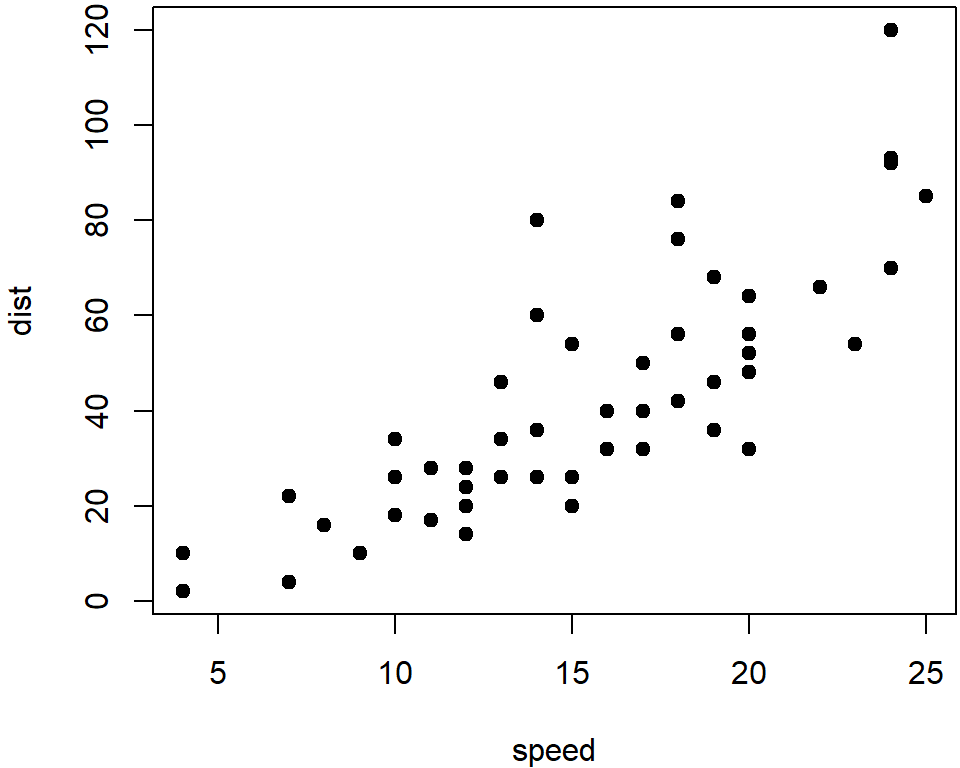
\includegraphics{0000-preciomedio_files/figure-latex/unnamed-chunk-5-1.pdf}

\end{col}

\begin{col}{0.05\textwidth}
~

\end{col}

\begin{col}{0.4\textwidth}
The figure on the left-hand side shows the \texttt{cars} data.

Lorem ipsum dolor sit amet, consectetur adipiscing elit, sed do eiusmod
tempor incididunt ut labore et dolore magna aliqua. Ut enim ad minim
veniam, quis nostrud exercitation ullamco laboris nisi ut aliquip ex ea
commodo consequat. Duis aute irure dolor in reprehenderit in voluptate
velit esse cillum dolore eu fugiat nulla pariatur.

\end{col}


\end{cols}

\begin{longtable}[]{@{}rrr@{}}
\toprule
orden & precio & unidades\tabularnewline
\midrule
\endhead
1 & 10 & 100\tabularnewline
\bottomrule
\end{longtable}

\begin{itemize}
\tightlist
\item
  \textbf{Coste} Coste medio de compra de las acciones
\item
  \textbf{Valor} Valor de la cartera al momento actual
\item
  \textbf{Neto} Precio que marca el punto de ruptura
\end{itemize}

Usamos el termino precio neto frente al mas correcto Precio Medio para
indicar cual es el precio de \textbf{venta} que me ofrece un beneficio
global de 0. Dicho de otro modo, el precio minimo al que puedo deshacer
la posicion sin perder dinero.

Supongamos que hago una primera operacion de compra:

Operaciones Posicion +----------+--------+-------+
+----------+--------+-------+------+\\
\textbar{} Unidades \textbar{} Precio \textbar{} Valor \textbar{}
\textbar{} Balance \textbar{} Precio \textbar{} Valor \textbar{} Neto
\textbar{} +----------+--------+-------+
+----------+--------+-------+------+ \textbar{} 10 \textbar{} 100
\textbar{} 1000 \textbar{} \textbar{} 10 \textbar{} 100 \textbar{} 1000
\textbar{} 100 \textbar{} +----------+--------+-------+
+----------+--------+-------+------+

La operacion es basica, logicamente si he comprado \textbf{n} unidades a
un precio \textbf{p}, si las vendo por debajo de ese precio pierdo
dinero, si lo vendo por encima de ese precio, gano dinero

Ahora supongamos que vendo 5 de mis unidades a 120

Opreraciones Posicion +----------+--------+-------+
+----------+--------+-------+------+\\
\textbar{} Unidades \textbar{} Precio \textbar{} Valor \textbar{}
\textbar{} Balance \textbar{} Precio \textbar{} Valor \textbar{} Neto
\textbar{} +----------+--------+-------+
+----------+--------+-------+------+ \textbar{} -5 \textbar{} 120
\textbar{} -600 \textbar{} \textbar{} 5 \textbar{} 100 \textbar{} 1000
\textbar{} 100 \textbar{} +----------+--------+-------+
+----------+--------+-------+------+

Ejemplo:

Operaciones\\
+------+----------+--------+--------+ \textbar{} Tipo \textbar{}
Unidades \textbar{} Precio \textbar{} Valor \textbar{}
+------+----------+--------+--------+ \textbar{} C \textbar{} 20
\textbar{} 100 \textbar{} 2000 \textbar{} \textbar{} V \textbar{} -10
\textbar{} 200 \textbar{} -2000 \textbar{}
+------+----------+--------+--------+

Con estas dos operaciones he obtenido un beneficio del 100\% y he
recuperado la inversion, con lo que el valor neto seria 0. Podria
regalar la inversion sin perder dinero.

Para evitar esto, introducimos el concepto de \textbf{regularizacion}

ESte es un registro que me marca el punto a partir del cual considerar
las operaciones posteriores. Tipicamente, y desde el punto de vista
contable, se genera un registro de regularizacion cada 1/1

Operaciones\\
+------+----------+--------+--------+ \textbar{} Tipo \textbar{}
Unidades \textbar{} Precio \textbar{} Valor \textbar{}
+------+----------+--------+--------+ \textbar{} C \textbar{} 20
\textbar{} 100 \textbar{} 2000 \textbar{} \textbar{} V \textbar{} -10
\textbar{} 200 \textbar{} -2000 \textbar{} \textbar{} R \textbar{} 10
\textbar{} 100 \textbar{} 2000 \textbar{} Usamos el precio medio de
compra +------+----------+--------+--------+

\end{document}
